Bitcoin which was 2008 introduced, is the more mature platform, compared to Ethereum. 
We want to give a short overview about both technologies and compare them. As the original paper is analyzing and describing the Bitcoin world. 
On the one hand we want to give some insights in the most important technologies on the blockchain market and also might gather some information about possible problems with the outcome. 

Let’s start with the data, by now the Bitcoin blockchain has the size of 197 gigabytes in the beginning of January its growing constantly, since it was introduced \cite{StatBit1}.
It takes on average 9,6 minutes to confirm a transaction at the end of February 2019 \cite{StatBit1}. 
The Bitcoin index value for the same period was 3.799,68 US Dollar, were the number of wallets grew over the last years constantly and reached 32 million wallet users at the end of 2018.

\begin{figure}[h]
  \centering
  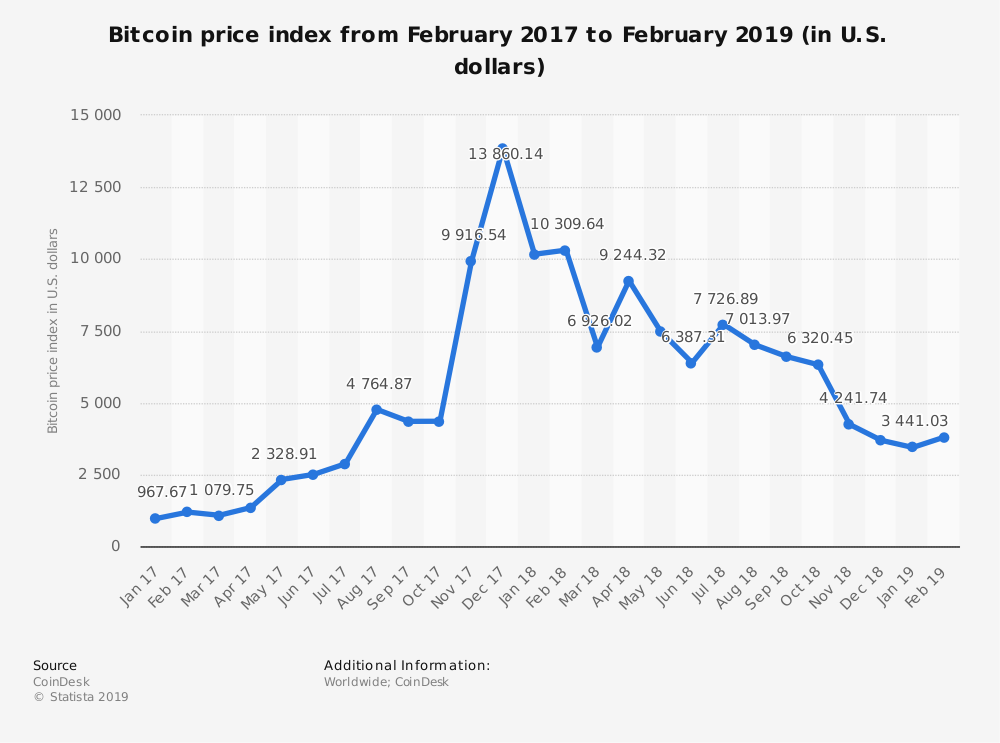
\includegraphics[width=\linewidth]{figures/marketBit.png}
  \caption{Bitcoin Price Index- \cite{statEthereum}}
  \label{fig:marketcapBitcoin}
\end{figure}


The market capitalization had a peak in Quarter four 2017 and it has since decreased, to a value of 66,18 million US Dollar in the end of 2018.
Compared the Ethereum already grew to the size of 181.65 GB, this represents the full blockchain size of all blocks. The average mining time is less that the Bitcoin, with 13.5 s per block \cite{BitInfoEther}. The number of wallets exceeded 50 million in the end of 2018 \cite{BitInfoBitcoin}.

\begin{figure}[h]
  \centering
  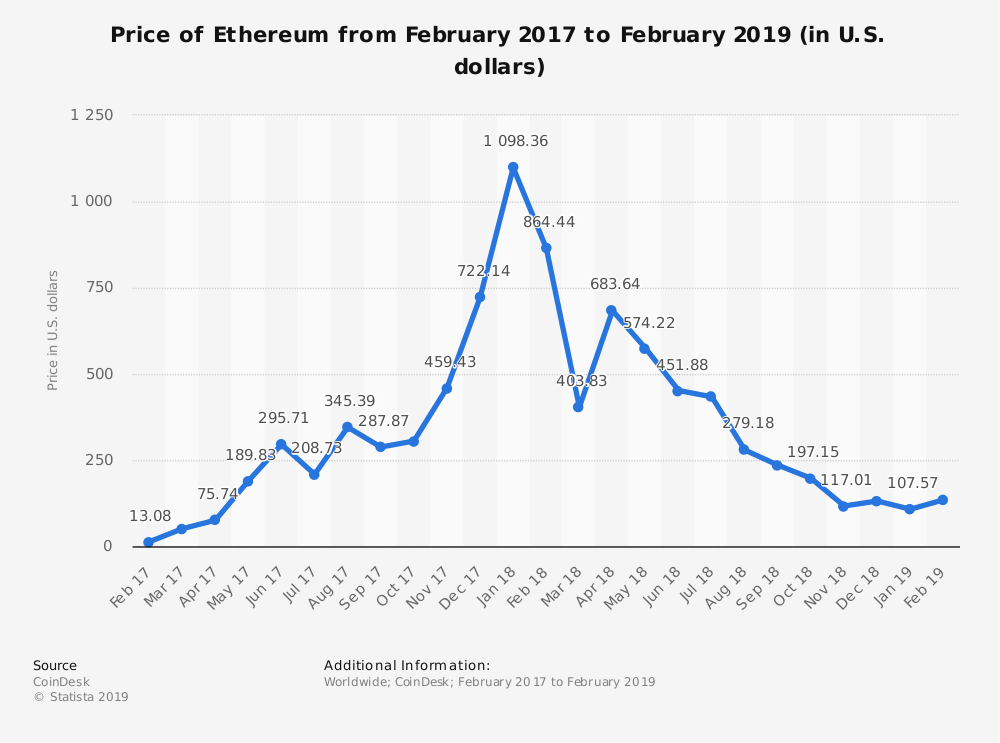
\includegraphics[width=\linewidth]{figures/EthereumPrice.png}
  \caption{Ethereum Price Development - \cite{statEthereum}}
  \label{fig:marketcapEthereum}
\end{figure}

Even if the wallets are increasing, the number of active addresses, referencing to BitInfoCharts, there are less active Ethereum addresses in 2018. 
The price of Ethereum is in the End of February 2019 amounted to 134,82 US Dollar \cite{StatPriceEther}.
Comparable to the Bitcoin, the peak was in 2017 and has been decreasing since then. 
Similar to the peak in price to most active period was in the end of 2017, here more than 1.13 million addresses were registered \cite{Partz2018}. In the End of 2018 there were only 328.400 active addresses recorded. 

The data can give some insights, but just in relation to the idea of both technologies they get more relevance. 
The most important difference is, that the idea behind the bitcoin was to create an independent currency.
That is not easy to manipulate and does not need an intermediary to be trusted. 
The community should be the verification, that no one would manipulate the blockchain. 
The technology was described in the former chapter. 
In contrast the Ethereum was developed afterwards. 
The person who wrote the white paper, Vitalik Butin, wanted to create more than a currency. \cite{vitalikwhite}
He got inspired by the technology behind the bitcoin and wanted to go beyond. 
That why he created a platform usable to write applications on, backed with the same technology. 
As described in the ‘Ethereum Theory’ chapter, along the way he also was able to improve some downsides about the bitcoin, introducing the merkle Patricia tree. 
Another advantage is that he made the platform able to work with a turin-complete language. 
In the End all that was necessary, as the Ethereum Blockchain has to deal with way more complexity when it wants to serve as a platform for applications.
